\documentclass[a4paper]{article}

\usepackage[english]{babel}
\usepackage[utf8]{inputenc}
\usepackage{amsmath}
\usepackage{graphicx}
\usepackage[colorinlistoftodos]{todonotes}
\usepackage{algorithm}
\usepackage{algorithmic}
\usepackage{listings}


\title{COMP90015 Distributed Systems \\Assignment 1: Multi-threaded Dictionary Server}

\author{ZHAOFENG QIU 1101584\\The University of Melbourne}

\date{\today}

\begin{document}
\maketitle

\section{Problem Context}
\label{sec:introduction}

In this project, a multi-threaded dictionary client-server system is designed and implemented using a client-server architecture. The server of the system allows concurrent clients to modify or query the remote dictionary by using thread-per-request architecture in the server. The system provides reliable communication between the server and clients by using TCP protocol. Also, JSON is used in the system for providing a message exchange protocol between the server and clients. As for failure handling, errors including I/O errors, Network Connection error, and parameters errors, are properly managed on both the server and the client side. Also, illegal requests (such as adding a word that is already in the dictionary, removing or querying a none-exit word and adding a word without meaning) from clients can be detected and handled by the server properly. Moreover, the server can handle concurrent requests at the same time and edit the data in a correct way.

\section{System Components} % (fold)
\label{sec:theory}
\subsection{Server}
The server is implemented using thread-per-request architecture and can detect and handle multiple failures. For every new request sent by clients, the server would create a new thread to handle it and give it a response. Since the server is using multi-thread technology, it can handle requests from different clients concurrently. However, when it comes to data modification, because the relative functions provided by the dictionary controller are synchronized, there will be no ambiguity in modifying the data in the dictionary. According to specific contexts, the server would handle requests in different ways and send back different states(which indicate the specific implementation) and feedbacks to clients. For better-exchanging messages with clients,  every response would be packed in JSON format before sending it back to clients. Besides, the length of word and meaning provided by users , the server provides a GUI for logging operations and showing information about the server.

\subsection{Client}
The client is mainly composed of two parts: the Client’s Controller and the Client’s GUI. It can detect and handle failures such as Network communication problems and Incorrect parameter input problems. The Client’s Controller part is responsible for handling the user’s operational requirements captured by the GUI. For each ADD, DELETE, QUERY operations given by the user, the controller would establish a new TCP connection with the server and would close it when the controller gets the response of it. In this case, the client would not check whether the server is running before processing the three operations given above. The GUI implemented with Swing can provide visual interfaces to users. In addition to satisfying the user’s query and modification operations, it also prompts the user how to use the client, such as asking them to enter a word before clicking the ADD button or REMOVE button, which can improve user’s experience.

\section{Design Details}
\subsection{Client Package}
The diagram of classes in the Client Package is shown in Figure 1.\\
\begin{figure}[H]
	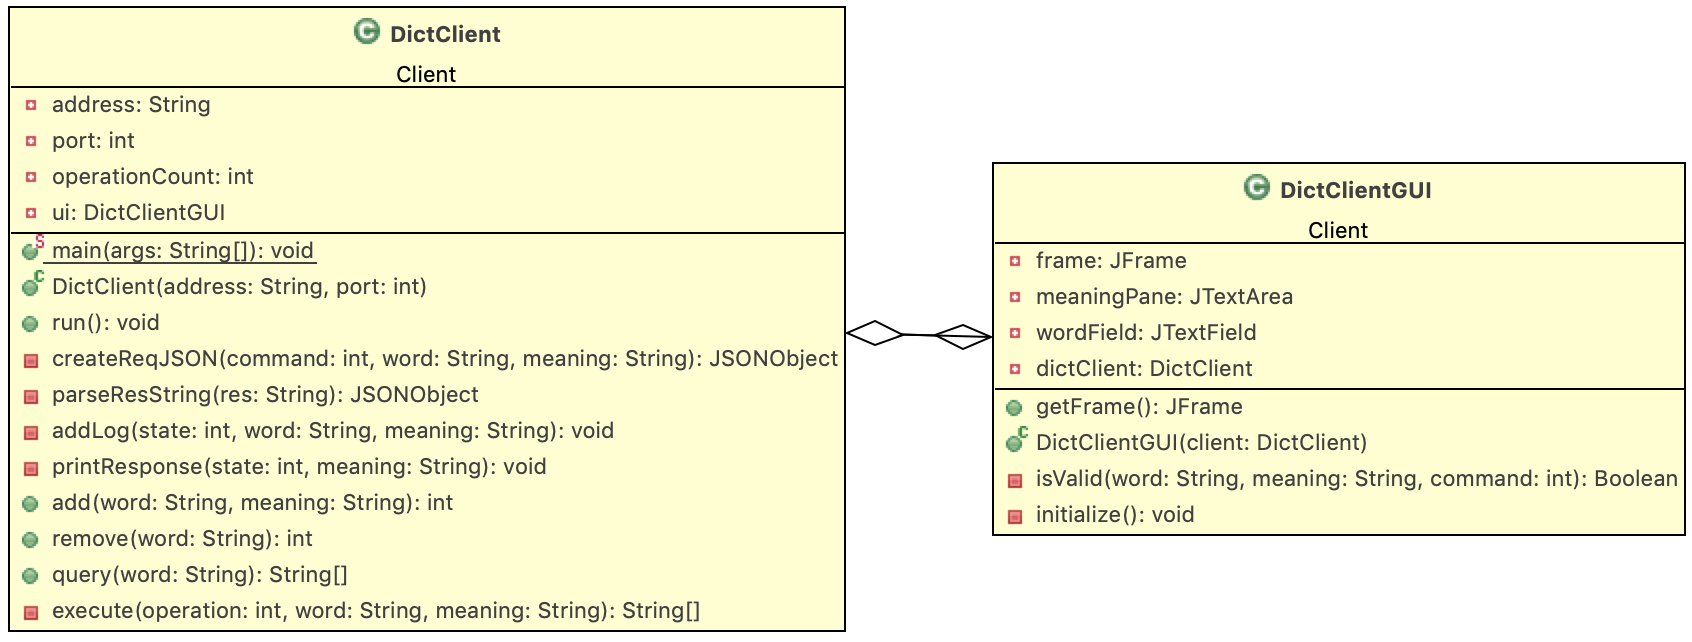
\includegraphics[width=\linewidth]{ClientUML.png}
	\caption{Client Package Class Diagram}
\end{figure}
When the client starts to run, it would first check whether the server's address and port are given. After that, it would check whether the formats of parameters are correct. Before the user executes any ADD, DELETE or QUERY operation, the client would not try to check and connect to the server.\par
When the user tries to execute any of the three operations, the client would first validate the integrity of the information need by the request. Then it would try to create a TCP connection with the server. If the client can not connect to the server, it would advise the user to restart the application with the proper address and port. \par
When they successfully connect, the client would create a request message in the JSON format shown in Table 1.

\begin{table}[H]
	\caption{Client request format (JSON fields)} 
	\begin{tabular}{|l|l|}
		\hline
		Command & A number indicating different command(detailed in table 3)   )                             \\ \hline
		Word & A word for operation                               \\ \hline
		Meaning  & The meaning of a word(Only need in ADD Command)\\ \hline
	\end{tabular}
\end{table}

Moreover, the client provides an adaptive window to users which can avoid the Out-Of-Bound text error. Also, some tips would show in the windows when a user tries to do some incorrect operation. The GUI is shown in Figure 2.

\begin{figure}[H]
	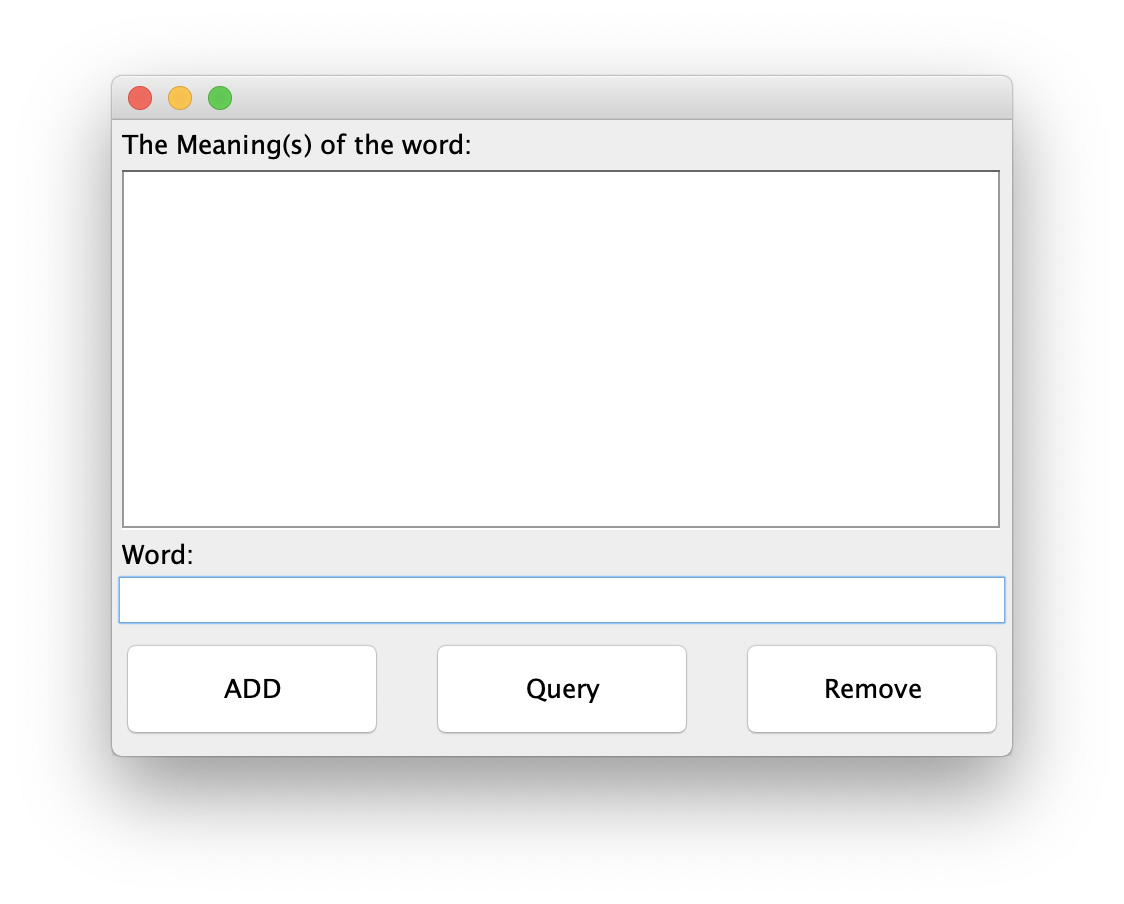
\includegraphics[width=\linewidth]{clientGUI.png}
	\caption{Client GUI}
\end{figure}
\newpage
\subsection{Server Package}
The diagram of classes in the Server Package is shown in figure 3.\\
\begin{figure}[H]
	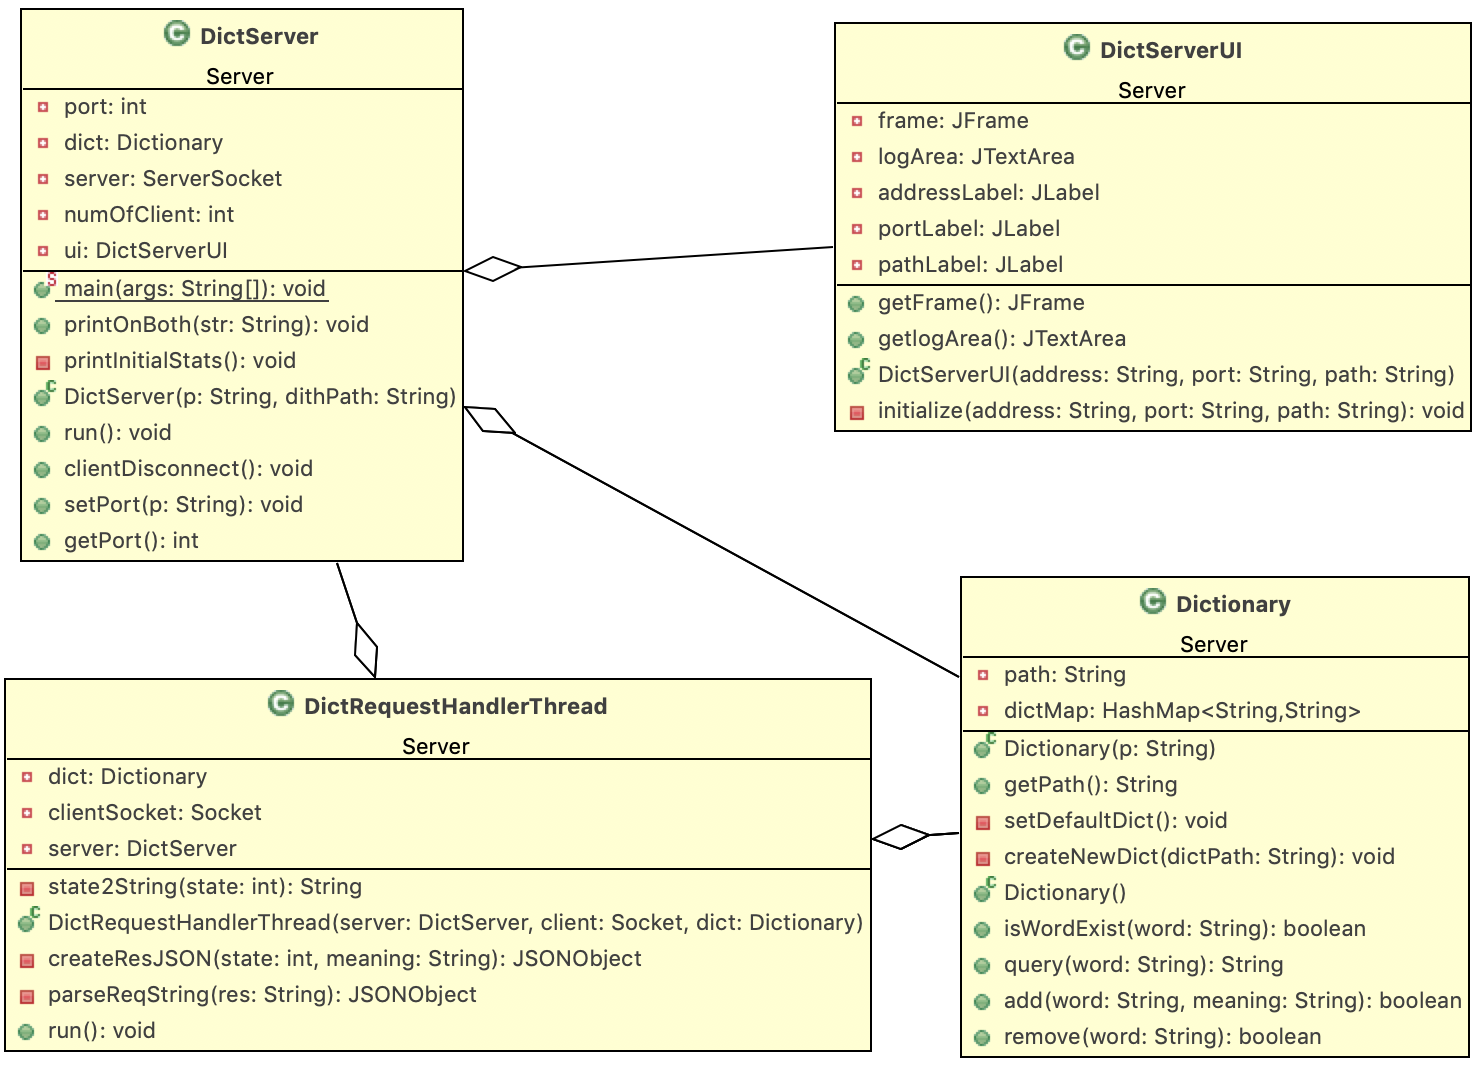
\includegraphics[width=\linewidth]{ServerUML.png}
	\caption{Server Package Class Diagram}
\end{figure}

When the server starts to run, it would first check whether the server's port and the dictionary's path are given. After that, it would check whether the formats of parameters are correct and try to read from the dictionary. If the giving dictionary doesn't exist or the format in the dictionary file is not valid, the server would create a default dictionary.

When the server receives a request from a client. It would create a thread to handle the request. According to distinct contexts, the server would handle requests in different ways and send back different states and feedbacks to clients. The response's JSON format is shown in Table 2.

\begin{table}[H]
	\caption{Server response format (JSON fields)}
	\begin{tabular}{|p{1.3cm}|p{10cm}|}
		\hline
		State & A number indicating the state (detailed in table 3)                            \\ \hline
		Meaning & The meaning of a word(Only need in QUERRY mode)                               \\ \hline
	\end{tabular}
\end{table}

Besides, the server also provides an adaptive window that can avoid the Out-Of-Bound text error. The use of it is to provide useful information about the server and recording the operation of the system. The GUI is shown in Figure 4.

\begin{figure}[H]
	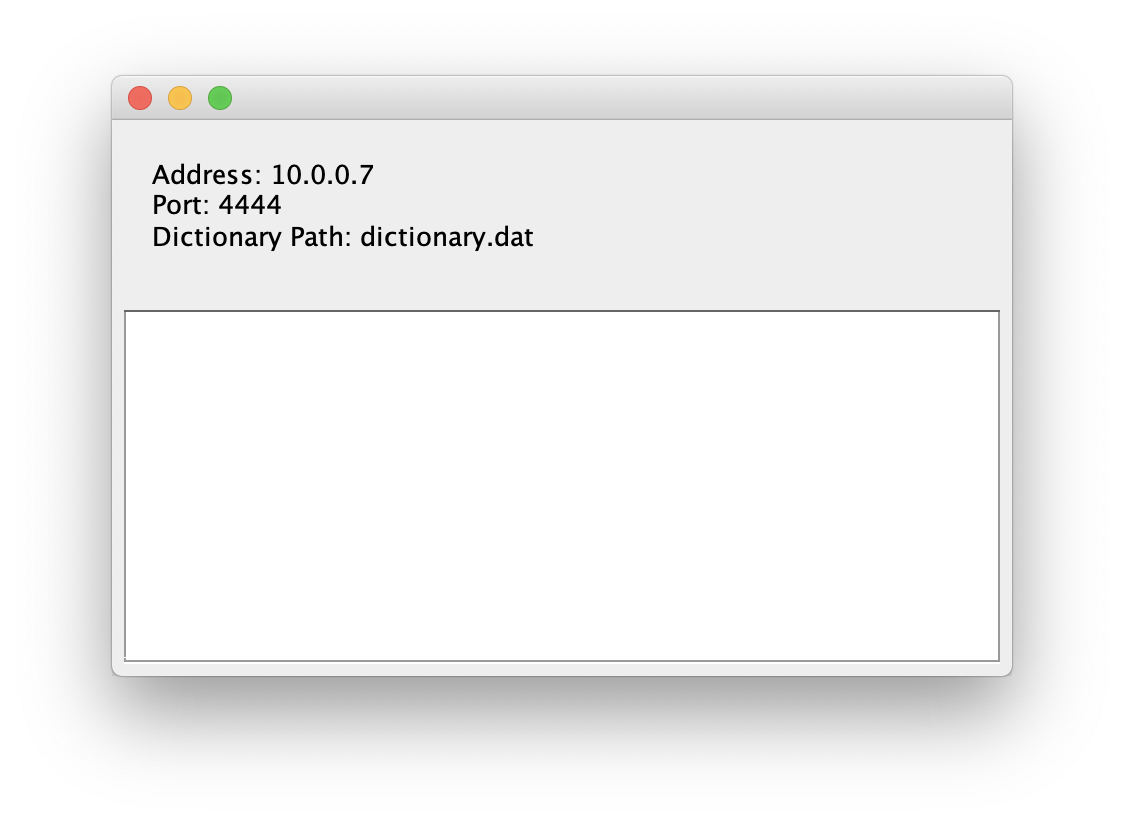
\includegraphics[width=\linewidth]{serverGUI.png}
	\caption{Server GUI}
\end{figure}

\subsection{StateCode Package}
The StateCode class is responsible for providing status code comparison tables shared by both the server and clients. The comparison tables is shown in Table3.
\begin{table}[H]
	\caption{Status code reference}
	\begin{tabular}{|p{0.6cm}|p{10.7cm}|}
		\hline
		0 & QUERY Command, used in request.\\ \hline
		1 & ADD Command, used in request.   \\ \hline
		2 & REMOVE command, telling the client the operation can not be executed. \\ \hline
		3 & Successful Operation, telling the client the operation is successfully executed.\\ \hline
		4 & Unsuccessful Operation, used in respones.\\ \hline
		403 & Connection Failure, used in connection.\\ \hline
	\end{tabular}
\end{table}
\subsection{Interaction Diagram}
The interaction diagram between a single client and the server is shown in Figure 5.
\begin{figure}[H]
	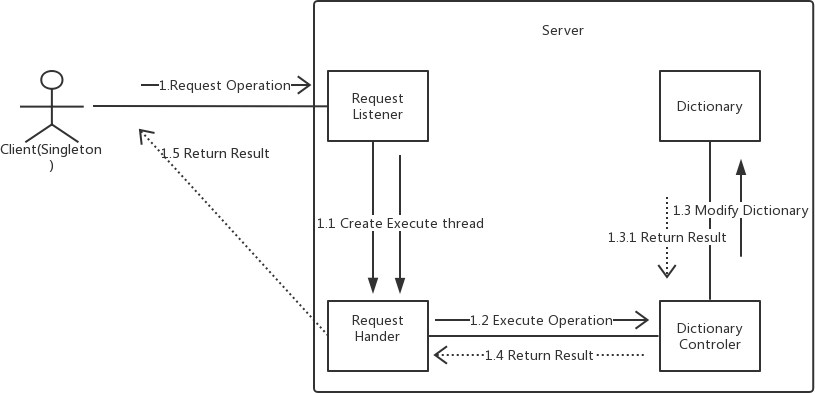
\includegraphics[width=\linewidth]{InteractionDiagram.png}
	\caption{Interaction Diagram}
\end{figure}

\section{Critical Analysis}
\subsection{Failure Handling and Recovery}
The two major errors that may occur in the system are operation errors and connection errors. For each kind of errors, the system has provided proper notification to help the users understand what goes wrong.
\begin{enumerate}
	\item \textit{Operation Errors}
	Operation errors occurs when the user started the program in the wrong way or performed the wrong operation. The problems and their solutions are listed in Table 4.
	\begin{table}[H]
		\caption{Operation errors and solution} 
		\begin{tabular}{|p{5.3cm}|p{6cm}|}
			\hline
			Description & Solution \\ \hline
			Inadequate startup paramaters (both sides) &  Prevent startup and show sample.\\ \hline
			Input invalid port number (both sides) &  Prevent startup and ask for valid port number.\\ \hline
			Empty input (client side) & Show GUI tips and ask for input.\\ \hline
			The dictionary file not exists (server side) &  Use default fictionary \\ \hline
			Default dictionary file not exists (server side) &  create default fictionary \\ \hline
			Get request to add a exist word (server side) & Send word-exist feedback to client \\ \hline
			Get request to query a non-exist word (server side) & Send word-non-exist feedback to client \\ \hline
			Get request to remove a non-exist word (server side) & Send word-non-exist feedback to client \\ \hline
		\end{tabular}
	\end{table}

	\item \textit{Connection Errors}
	In the real world, the network is unstable. Besides, the server may not work, and the port may be wrong. The problems and their solutions are listed in Table 5.

	\begin{table}[H]
		\caption{Connection errors and solution} 
		\begin{tabular}{|p{5.3cm}|p{6cm}|}
			\hline
			Description & Solution \\ \hline
			Connection Timed Out (client sides)& Show GUI tips and ask for a connectable server. \\ \hline
			Connectionless Port (client sides)  &  Show GUI tips and ask for a connectable port.\\ \hline
		\end{tabular}
	\end{table}
\end{enumerate}
\subsection{Analysis of the System}
\subsubsection{Advantage}
\begin{enumerate}
\item \textit{Scalability}
Based on the feature that users operate infrequently in dictionary application, using Thread-per-request scales better than thread-per-connection. Java threads are rather expensive, typically using a 1Mb memory segment each, whether they are active or idle. In the thread-per-request model, the thread is only associated while a request is being processed. That usually means that the service needs fewer threads to handle the same number of users. And since threads use significant resources, that means that the service will be more scalable.

\item \textit{Heterogeneity}
Using Java to implement both the server can solve the problem of heterogeneity. This is because JVM provides basic cross-platform.

\item \textit{Notification of Error}
Most of the errors which may occur during the using period have been handle properly. Through giving feedback on the GUI, users can easily find out the error.
\end{enumerate}

\subsubsection{Disadvantage}
\begin{enumerate}
\item \textit{Problem of thread-per-request}
It is expensive to create a new thread for each request. The server that creates a new thread for each request may spend more time and system resources on creating and destroying threads than it spends on processing actual user requests. Using worker pool architecture can solve the problem.

\item \textit{Security Concern}
Since access to the server is unrestricted, every one can send a request to the server. And there is no data format check on the request. The server can be easily attacked. There is a need to guarantee the privacy, integrity of resources in the server. Besides, the length and the format of word and meaning provided by users would not be check, which may also cause errors.
\end{enumerate}

\subsection{Creativity elements}
\begin{enumerate}
\item \textit{Server GUI}
A GUI for managing the server is provided. The use of it is to provide useful information about the server and recording the operation of the system. The GUI is shown in Figure 4.

\item \textit{Timeout Handler}
In the real world, the network is unstable. Adding timeout mechanism can effectively avoid the problem of program jamming. The relative class's Class Diagram is shown in Figure 6.
\begin{figure}[H]
	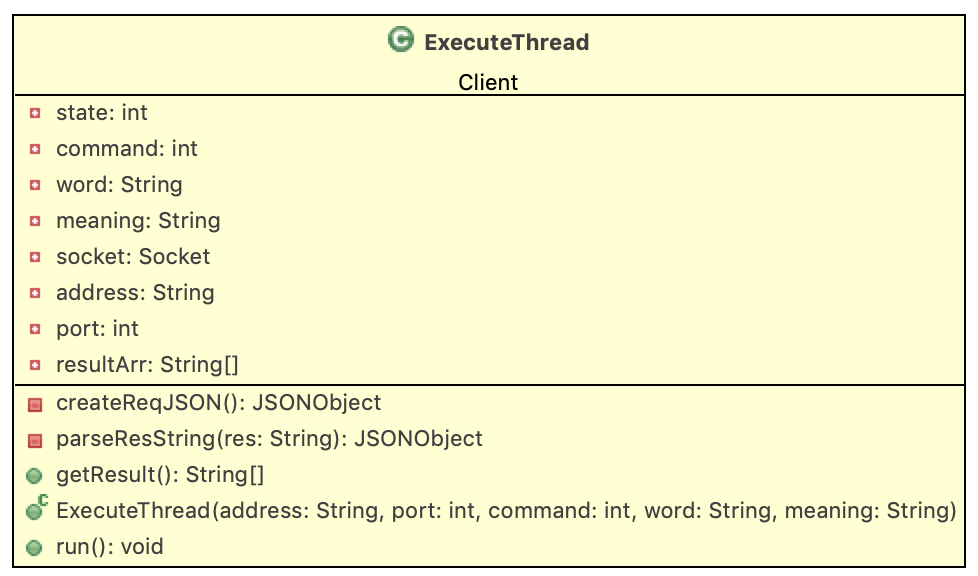
\includegraphics[width=\linewidth]{timeoutUML.png}
	\caption{TimeoutClass Class Diagram}
\end{figure}

\item \textit{Adaptive GUI}
Adaptive GUI to users which can avoid the Out-Of-Bound text error are provided on both the server and clients sides. 

\end{enumerate}
\end{document}













